% ============================================================================
%  Artigo — Text Mining, Opção 2: Deteção de Notícias Falsas (Fake.Br)
%  Modelo oficial Springer LNCS (llncs.cls + splncs04.bst). NÃO alterar margens,
%  tipos de letra nem espaçamentos (regra do enunciado).
%  Limite: 25 páginas SEM contar referências e anexos.
%  Compilar:  latexmk -pdf main.tex     (ou no Overleaf: carregar a pasta paper/)
%  As tabelas em tables/ são GERADAS por src/make_tables.py — não editar à mão.
% ============================================================================
\documentclass[runningheads]{llncs}

\usepackage[T1]{fontenc}
\usepackage[utf8]{inputenc}
\usepackage[portuguese]{babel}
\usepackage{graphicx}
\usepackage{booktabs}
\usepackage{xcolor}
\usepackage{url}
\usepackage{hyperref}
\hypersetup{colorlinks=true, linkcolor=blue, citecolor=blue, urlcolor=blue}

% Marcador de trabalho por fazer. Para a versão final: trocar por \newcommand{\todo}[1]{}
% e confirmar que não sobra nenhum (procurar "TODO" no PDF).
\newcommand{\todo}[1]{}
\newcommand{\repo}{\url{https://github.com/hugo7979/fakebr-tm}}

\begin{document}
\renewcommand{\andname}{e}\renewcommand{\lastandname}{\unskip\ e}

\title{Deteção de notícias falsas no corpus Fake.Br}
\titlerunning{Deteção de notícias falsas no corpus Fake.Br}

\author{Diogo Filipe Oliveira Gomes (PG63946) \and Sérgio Paulo Vieira Carvalho (PG63711) \and
        Hugo Novais Martins (PG64175) \and Diogo Valério Borges (PG64174) \and
        Tiago Alexandre Lopes Mendes (PG64031)}
\authorrunning{D. Gomes, S. Carvalho, H. Martins, D. Borges e T. Mendes}
\institute{Departamento de Informática, Universidade do Minho, Braga, Portugal\\
\email{\{pg63946,pg63711,pg64175,pg64174,pg64031\}@alunos.uminho.pt}}

\maketitle

% Resumo: 150 a 250 palavras (enunciado). Rever no fim, com os números do TESTE.
\begin{abstract}
Um projeto de verificação de factos precisa de priorizar notícias suspeitas sem as ler uma a uma.
Estudamos que características linguísticas distinguem notícias falsas de verdadeiras em português
e se um detetor generaliza para temas não vistos, usando o corpus Fake.Br (7\,200 notícias
emparelhadas por assunto). Construímos um pipeline completo com divisão de teste agrupada por par,
para evitar fugas de informação, e três tarefas: classificação, modelação de tópicos e extração de
entidades. Mostramos que o corpus tem um atalho forte: um classificador que usa apenas o comprimento
do texto obtém F1-macro de 0,944 em validação cruzada, perto dos 0,974 do melhor modelo TF-IDF.
Descobrimos ainda que a versão normalizada do corpus cria um segundo atalho: as notícias
verdadeiras acabam quase sempre a meio de uma frase, e o último carácter basta para 0,890. Numa versão
sem os dois atalhos, os n-gramas de caracteres obtêm 0,939 e o BERTimbau afinado 0,987 no teste, e a remoção
de \emph{stopwords} e o \emph{stemming} pioram os resultados, o que indica que o sinal está no
estilo e não no vocabulário temático. Os tópicos LDA estão mais associados
ao tema (NMI 0,104) do que à veracidade (NMI 0,047), e, segundo 100 notícias anotadas manualmente, as verdadeiras
contêm cerca de cinco vezes mais datas. Os modelos de estilo perdem menos desempenho em temas não vistos
do que os de palavras. Discutimos o viés de fonte do corpus (93\% das notícias falsas vêm de um
único sítio), as implicações éticas e um conjunto de recomendações para a organização.
\keywords{Notícias falsas \and Português \and Estilometria \and Modelação de tópicos \and Extração de informação}
\end{abstract}

% Responsável: P1 (revisão final: todos)
\section{Introdução}\label{sec:intro}

\paragraph{O problema da organização.}
Uma equipa de verificação de factos recebe diariamente mais notícias do que consegue verificar.
Precisa de uma ferramenta que \emph{ordene} as notícias por suspeição, para que os verificadores
humanos comecem pelas mais prováveis de serem falsas. A ferramenta não decide o que é falso: apoia
a triagem. Esta distinção condiciona a escolha de métricas (o custo de um falso negativo e de um
falso positivo) e as considerações éticas (Secção~\ref{sec:etica}).

\paragraph{Pergunta de investigação.}
\emph{Que características linguísticas distinguem as notícias falsas das verdadeiras num corpus real
em português, e um detetor treinado com elas mantém o desempenho quando (a) se neutraliza o
comprimento dos textos e (b) é aplicado a temas que não viu no treino?}

\paragraph{Critério de sucesso (fixado antes de usar o teste).}
A pergunta considera-se respondida se: (i) identificarmos atributos com diferenças entre classes
estatisticamente significativas e interpretáveis; (ii) um modelo baseado no conteúdo superar a
\emph{baseline} que usa apenas o comprimento, com intervalos de confiança a 95\% não sobrepostos;
e (iii) quantificarmos a queda de desempenho em temas não vistos face ao desempenho no mesmo tema.

\paragraph{Contribuições.}
\begin{enumerate}
\item Um protocolo de avaliação para o Fake.Br sem fugas de informação: divisão agrupada por par de
notícias e por textos repetidos entre pares (Secção~\ref{sec:config}).
\item A evidência de que o comprimento, sozinho, explica a maior parte do desempenho reportado em
textos completos, e uma comparação de representações quando esse atalho é removido.
\item Uma análise convergente com três tarefas (classificação, tópicos e extração de entidades) que
aponta o \emph{estilo} e a \emph{ancoragem factual} (datas, locais) como os sinais robustos, e não o tema.
\item Um repositório que reproduz a tabela principal com um único comando: \repo.
\end{enumerate}

O resto do artigo está organizado assim: a Secção~\ref{sec:rel} discute o trabalho relacionado; a
\ref{sec:dados} caracteriza o corpus; as Secções~\ref{sec:metodo} e~\ref{sec:config} descrevem o
método e a configuração experimental; a \ref{sec:resultados} apresenta os resultados, discutidos na
\ref{sec:discussao}; a \ref{sec:etica} trata as questões éticas e as limitações, e a
\ref{sec:conclusao} conclui.

% Responsável: P1 + P2. Enunciado: >= 8 referências, COMENTADAS CRITICAMENTE (não só enumeradas).
% Factos verificados nos resumos/textos dos artigos em 17/11/2026 (Potthast, Pérez-Rosas, Horne & Adalı,
% Santos et al.). Ler os artigos completos antes da apresentação.
\section{Trabalho relacionado}\label{sec:rel}

\paragraph{Panoramas.}
Shu et~al.~\cite{shu2017} e Zhou e Zafarani~\cite{zhou2020} organizam a deteção de notícias falsas
em abordagens baseadas no conteúdo (conhecimento e estilo), na propagação e na fonte. O nosso
trabalho situa-se na deteção pelo \emph{estilo} do conteúdo, a única possível quando, como no
cenário da organização, só se dispõe do texto. A nossa análise de erros confirma a fragilidade que
estes panoramas apontam a esta família de métodos: basta imitar a escrita jornalística para enganar
o detetor.

\paragraph{Estilo e notícias falsas.}
Horne e Adal{\i}~\cite{horne2017} concluíram que, em inglês, as notícias falsas se parecem mais com
a sátira do que com notícias reais, que a estrutura do título e o uso de nomes próprios as distinguem
e que persuadem por heurísticas, dirigindo-se a leitores que não passam do título. Potthast
et~al.~\cite{potthast2018} mostraram que o estilo separa bem notícias hiperpartidárias das restantes
(F1 de 0,78) e a sátira de ambas (0,81), mas que a deteção de notícias falsas apenas pelo estilo
falha (F1 de 0,46). A diferença face aos valores próximos de 0,95 no Fake.Br é instrutiva: quando as
notícias falsas vêm de poucos sítios, o estilo da fonte confunde-se com a falsidade. Pérez-Rosas
et~al.~\cite{perezrosas2018} construíram dois conjuntos em inglês (FakeNewsAMT e Celebrity) e
combinaram atributos lexicais, sintáticos e de legibilidade; ao treinar num domínio e testar no
outro, a exatidão desceu de 0,67--0,78 para 0,51--0,61. No nosso protocolo por tema a queda é muito
menor (até 5,5 pontos), possivelmente porque as fontes são as mesmas em todos os temas.

\paragraph{Notícias falsas em português.}
Monteiro et~al.~\cite{monteiro2018} criaram o Fake.Br: 3\,600 notícias falsas e 3\,600 verdadeiras,
alinhadas por assunto e recolhidas entre janeiro de 2016 e janeiro de 2018, com 89\% de exatidão
usando SVM sobre \emph{bag-of-words}; atributos como a pausalidade e a emotividade, sozinhos, ficaram
perto de 55\%~\cite{santos2020}. Silva et~al.~\cite{silva2020} disponibilizaram o conjunto
publicamente e compararam vários métodos de aprendizagem automática, conjuntos de atributos e
classificadores. Santos et~al.~\cite{santos2020} mostraram que atributos de legibilidade, sozinhos,
chegam a 92\% de exatidão, com SVM e validação cruzada de 5 folds. Estes trabalhos estabeleceram o
corpus e as referências de desempenho, mas não indicam se as duas notícias de cada par ficam no mesmo
fold, nem quanto do desempenho se explica pelo comprimento ou pela forma como os textos acabam. São
estas as questões que o nosso protocolo controla: dividimos por par, medimos as \emph{baselines} de
comprimento e de final do texto e testamos temas não vistos.

\paragraph{Representações e avaliação.}
Usamos TF-IDF~\cite{manning2008} e o BERTimbau~\cite{souza2020}, uma variante do BERT~\cite{devlin2019}
pré-treinada em português do Brasil. Para os tópicos usamos LDA~\cite{blei2003}, avaliado com a
coerência NPMI, que Röder et~al.~\cite{roder2015} identificaram como uma das medidas mais
correlacionadas com o julgamento humano. Kapoor e Narayanan~\cite{kapoor2023} documentam como a
fuga de informação entre treino e teste inflaciona resultados em muitas áreas; no Fake.Br, o
emparelhamento das notícias torna esse risco concreto.

% Responsável: P1 (corpus) + P5 (anotação)
\section{Dados}\label{sec:dados}

\paragraph{Origem e licença.}
O Fake.Br~\cite{monteiro2018} contém 7\,200 notícias em português do Brasil: 3\,600 falsas e
3\,600 verdadeiras. Segundo os autores, as falsas foram recolhidas em sítios que as agregam e,
para cada uma, foi procurada manualmente uma notícia verdadeira sobre o mesmo assunto em jornais de
referência, formando pares. As notícias foram recolhidas entre janeiro de 2016 e janeiro de
2018~\cite{santos2020}. O corpus é
distribuído num repositório público\footnote{\url{https://github.com/roneysco/Fake.br-Corpus}}
que \textbf{não inclui ficheiro de licença}; os autores pedem apenas a citação dos artigos.
Usamo-lo para investigação, sem redistribuir os textos: o nosso código descarrega-o num
\emph{commit} fixo (\texttt{780f551}).

\paragraph{Estrutura.}
Cada notícia tem duas versões: o texto completo e uma versão em que o texto mais longo de cada
par foi cortado ao comprimento do mais curto. Acompanham-na 25 metadados (autor, ligação, categoria,
data e atributos linguísticos calculados pelos autores). Os temas são muito desequilibrados:
política (58\%), TV e celebridades (21\%), sociedade e quotidiano (18\%), e três temas pequenos
(ciência e tecnologia, economia, religião) que agregámos em ``outros'' (3\%).

\begin{table}[t]\centering\small
\caption{Estatísticas descritivas do conjunto de desenvolvimento (2\,878 pares).}\label{tab:corpus}
\begin{tabular}{lrr}
\toprule
& Verdadeiras & Falsas \\
\midrule
Documentos & 2 878 & 2 878 \\
Palavras (total) & 3 170 854 & 528 398 \\
Palavras por doc.\ (mediana) & 919 & 156 \\
\quad percentil 10 & 439 & 83 \\
\quad percentil 90 & 1 987 & 306 \\
Palavras, versão normalizada (mediana) & 157,5 & 155,0 \\
Palavras em maiúsculas (mediana) & 9 & 3 \\
Erros ortográficos (\%, média) & 0,22 & 0,38 \\
Palavras por frase (mediana) & 20,6 & 14,9 \\
Domínio mais frequente (\% da classe) & 64,3 & 92,7 \\
\bottomrule
\end{tabular}\par\smallskip{\footnotesize Metadados de estilo calculados pelos autores do corpus sobre o texto completo.}
\end{table}


\paragraph{Dificuldades.}
A Tabela~\ref{tab:corpus} e uma análise dos finais dos textos mostram quatro problemas que condicionam todo o trabalho.
(1)~\emph{Viés de comprimento}: as verdadeiras têm mediana de 919 palavras e as falsas de 156;
na versão normalizada as medianas ficam em 158 e 155. (2)~\emph{Viés de fonte}: 92,7\% das falsas
do conjunto de desenvolvimento vêm de um único domínio e 64,3\% das verdadeiras do G1.
(3)~\emph{Ruído e duplicação}: 17 notícias verdadeiras aparecem em mais do que um par (mesma
ligação), quatro ficheiros da versão normalizada não correspondem aos da versão completa
(numeração diferente) e as datas surgem em formatos heterogéneos. As falsas têm em média mais
erros ortográficos (0,38\% vs.\ 0,22\%) e frases mais curtas (14,9 vs.\ 20,6 palavras).
(4)~\emph{Artefacto de truncagem}: a versão normalizada, criada para remover o viés de comprimento,
cria outro. Como é quase sempre a verdadeira que é mais longa, 98\% das verdadeiras foram cortadas a
meio de uma frase, e só 7\% acabam em pontuação, contra 77\% das falsas. Quatro atributos sobre o
último carácter dão F1-macro de 0,890 (Tabela~\ref{tab:cv}). Criámos por isso uma terceira versão,
\emph{cortada}: as primeiras 100 palavras do texto normalizado (ou todas menos as 5 últimas, nos
textos mais curtos), de modo que \emph{todos} os textos terminam a meio e a mesma
\emph{baseline} desce para 0,395.

\paragraph{Lei de Zipf.}
A Figura~\ref{fig:zipf} mostra a frequência das palavras em função da ordem, em escala log-log.
Ajustando uma reta nas ordens 10 a 10\,000 obtemos $\alpha=1{,}130$ para as verdadeiras e
$\alpha=1{,}122$ para as falsas, próximos do valor clássico $\alpha\approx1$~\cite{zipf1949,piantadosi2014}.
As duas classes seguem a lei de forma quase idêntica; a diferença de vocabulário (74\,782 vs.\ 30\,804
tipos) resulta sobretudo da diferença de volume de texto. Cerca de 40\% do vocabulário são
\emph{hapax legomena}, o que justifica ignorar termos que ocorrem num só documento.

\begin{figure}[t]\centering
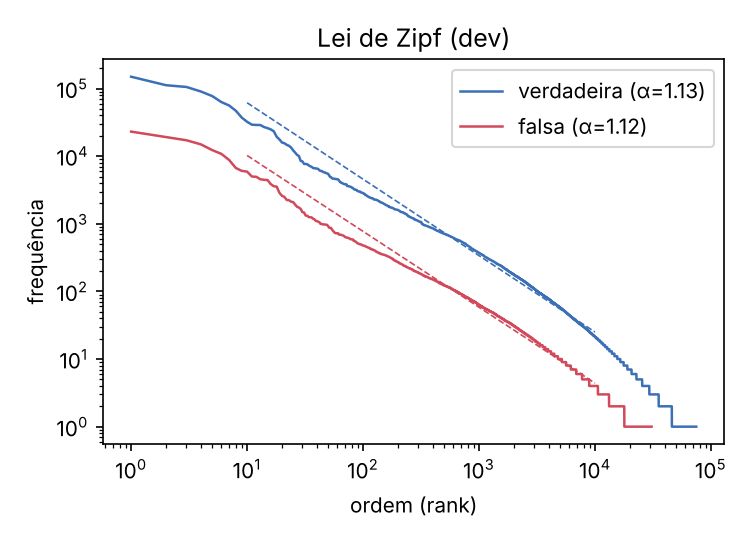
\includegraphics[width=0.48\linewidth]{figs/zipf.png}\hfill
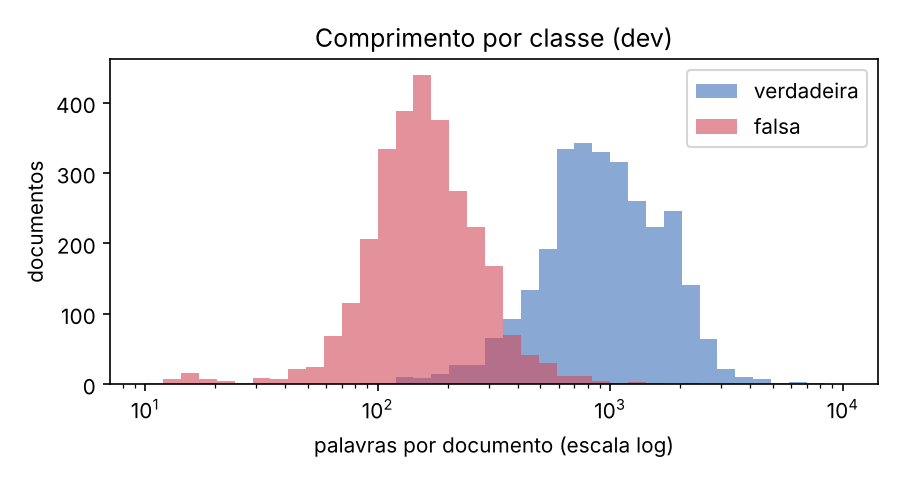
\includegraphics[width=0.48\linewidth]{figs/comprimento.png}
\caption{Esquerda: lei de Zipf por classe (dev), com a reta ajustada. Direita: distribuição do
comprimento por classe (escala logarítmica), que evidencia o viés de comprimento.}\label{fig:zipf}
\end{figure}

\paragraph{Anotação manual para a extração de informação.}
Selecionámos 50 pares (100 notícias) do conjunto de desenvolvimento, estratificados por tema,
usando o texto normalizado. Os anotadores não conhecem o rótulo de cada notícia (códigos opacos,
ordem aleatória) nem usam ferramentas de pré-anotação. Anotam quatro tipos: pessoa, organização,
local e data, segundo um guia com regras e exemplos (no repositório). Vinte notícias foram
anotadas por dois anotadores, para medir a concordância. Uma limitação: como os textos normalizados
das verdadeiras acabam quase sempre a meio de uma frase, o corte pode sugerir a classe ao anotador;
as regras de anotação não dependem da classe, e os anotadores foram instruídos a ignorá-la.
Ao longo da anotação surgiram casos não previstos (títulos como ``Dona'' ou ``Papa'', hospitais e
fazendas, partidos com a sigla do estado, horas), decididos em grupo e acrescentados ao guia antes de
todos terminarem. Os cinco anotadores produziram 931 entidades distintas no ouro principal. Nas 20
notícias com dupla anotação, a concordância (F1 entre anotadores) é de 0,875 com correspondência
estrita e 0,931 relaxada; é mais baixa nas datas (0,708 estrita, 0,958 relaxada), sobretudo por
diferenças na extensão da expressão (``quinta-feira, 18'' vs.\ ``quinta-feira''), e nas organizações
(0,816). Não houve adjudicação: o ouro de cada notícia é o do anotador principal. Uma verificação
automática de formato encontrou 10 inconsistências (cerca de 1\%: erros de cópia, como ``Mendonza''
por ``Mendoza'', e números de dia anotados sozinhos), que mantivemos como parte do ruído da anotação.

% Responsável: P2 (pré-processamento, clássicos) + P3 (BERTimbau) + P4 (tópicos) + P5 (EI)
\section{Metodologia}\label{sec:metodo}

\paragraph{Pré-processamento.}
Tokenizamos com uma expressão regular que mantém letras acentuadas e palavras hifenizadas
(``lava-jato'', ``quarta-feira'') e substitui ligações por um símbolo único. Os passos seguintes
são opcionais, para os podermos avaliar: minúsculas, remoção de \emph{stopwords} (lista do NLTK)
e \emph{stemming} RSLP~\cite{orengo2001}. A Tabela~\ref{tab:vocab} mostra o efeito no vocabulário:
as minúsculas reduzem-no 15\% e o RSLP 59\%; as \emph{stopwords} quase não alteram o vocabulário,
mas eliminam 42\% dos \emph{tokens}. A escolha final é feita pela \emph{ablation}
(Secção~\ref{sec:resultados}), não por convenção.

\begin{table}[t]\centering\small\setlength{\tabcolsep}{10pt}
\caption{Efeito de cada passo de pré-processamento no vocabulário (dev, texto completo).}\label{tab:vocab}
\begin{tabular}{lrrrr}
\toprule
Pipeline & Tokens & Vocabulário & Hapax & Redução (\%) \\
\midrule
Tokens originais & 3\,699\,252 & 94\,706 & 38\,235 & 0,0 \\
+ minúsculas & 3\,699\,252 & 80\,254 & 30\,483 & 15,3 \\
+ remoção de stopwords & 2\,135\,003 & 80\,065 & 30\,478 & 15,5 \\
+ stemming RSLP & 2\,135\,003 & 38\,489 & 14\,618 & 59,4 \\
\bottomrule
\end{tabular}
\end{table}


\paragraph{Representações.}
(i)~\emph{Comprimento}: o logaritmo do número de palavras, como \emph{baseline} informativa.
(ii)~\emph{Estilo}: os 20 atributos fornecidos com o corpus, e um subconjunto de 6 proporções que
não dependem diretamente do comprimento (pausalidade, comprimento médio de frase e de palavra,
erros ortográficos, emotividade e diversidade). (iii)~\emph{TF-IDF de palavras} (uni e bigramas,
TF sublinear, $\mathit{min\_df}=2$). (iv)~\emph{TF-IDF de caracteres} (2 a 5, dentro das palavras),
que capta grafia, morfologia e pontuação. (v)~\emph{BERTimbau}~\cite{souza2020}: média dos vetores
da última camada com o modelo congelado, e \emph{fine-tuning} completo.
O \emph{fine-tuning} usa 3 épocas, taxa de aprendizagem $2\times10^{-5}$ com aquecimento linear,
lotes de 16 e até 384 \emph{tokens}, reiniciando o modelo em cada fold.
Cada representação é avaliada sobre três versões do texto: completo, normalizado e cortado
(Secção~\ref{sec:dados}).

\paragraph{Classificadores.}
Regressão logística e SVM linear (\texttt{scikit-learn}~\cite{pedregosa2011}); a \emph{baseline}
mínima é a classe maioritária. Escolhemos modelos lineares por serem rápidos, robustos em espaços
esparsos e interpretáveis (pesos por atributo). Pusemos de lado, à partida e sem as testar,
as árvores de decisão e as florestas aleatórias, que lidam mal com dezenas de milhares de atributos
esparsos e são mais lentas, e o Naive Bayes multinomial, cuja hipótese de independência entre
atributos é pouco realista com n-gramas de caracteres sobrepostos.

\paragraph{Palavras distintivas.}
Para descrever o vocabulário de cada classe usamos o \emph{log-odds} com prior de Dirichlet
informativo~\cite{monroe2008}, que, ao contrário da frequência relativa, não sobrevaloriza
palavras raras.

\paragraph{Modelação de tópicos.}
Aplicamos LDA~\cite{blei2003} a contagens de palavras do texto normalizado, sem \emph{stopwords} nem
números (aqui interessa o conteúdo, não o estilo). Escolhemos o número de tópicos $K$ pela coerência
NPMI média dos 10 termos mais prováveis~\cite{roder2015}, com três sementes por $K$.

\paragraph{Extração de informação.}
Pessoas, organizações e locais são extraídos com o modelo \texttt{pt\_core\_news\_md} do spaCy
(as etiquetas \texttt{MISC} são ignoradas); as datas, que o modelo não etiqueta, são extraídas com
expressões regulares (datas completas, dias da semana, meses e anos). Duas regras de
pós-processamento alinham o extrator com o guia de anotação: nos padrões partido-estado
(``PSDB-MG'') fica só o partido, e ``Janeiro'' em ``Rio de Janeiro'' não conta como mês. Medimos também expressões de
atribuição de fontes (``segundo'', ``de acordo com'', ``disse'', ``afirmou''). A avaliação é feita
ao nível do documento: o conjunto de entidades distintas previsto é comparado com o anotado, com
correspondência estrita e relaxada (uma forma contém a outra, mesmo tipo).
Comparámos os três modelos de português do spaCy (\texttt{sm}, 16\,MB; \texttt{md}, 54\,MB;
\texttt{lg}, 631\,MB): processam todos cerca de 70 documentos por segundo em CPU, e o F1 global no
ouro sobe de 0,645 (\texttt{sm}) para 0,681 (\texttt{md}) e 0,697 (\texttt{lg}). Usamos o
\texttt{md} como compromisso entre qualidade e tamanho.

% Responsável: P2
\section{Configuração experimental}\label{sec:config}

\paragraph{Divisão desenvolvimento/teste.}
Antes de qualquer modelo, separámos 20\% dos dados para teste. A unidade de divisão é o
\emph{grupo}: o par de notícias, juntando os pares que partilham um texto ou uma ligação
(18 grupos com mais de um par). Usamos \texttt{StratifiedGroupKFold} (semente 42), estratificando
pelo tema. Resultam 5\,756 documentos de desenvolvimento e 1\,444 de teste, com zero grupos
partilhados. Sem este agrupamento, a notícia verdadeira de um par poderia ficar no treino e a
falsa no teste, e o modelo aproveitaria o assunto conhecido~\cite{kapoor2023}. A divisão está
guardada em \texttt{data/split.json} e é igual para todos os modelos.

\paragraph{Validação cruzada e métricas.}
Todas as escolhas (representação, hiperparâmetros, número de tópicos $K$ e passos de pré-processamento) foram tomadas com
validação cruzada de 5 folds, também agrupada, no desenvolvimento. Reportamos F1-macro (média e desvio-padrão entre folds), F1 por classe e o intervalo de confiança
a 95\% calculado com 1\,000 reamostragens \emph{bootstrap} das previsões \emph{out-of-fold}.
O teste é usado uma única vez, no fim,
com as configurações fixadas, e aí reportamos também a matriz de confusão.

\paragraph{Generalização por tema.}
Num protocolo \emph{leave-one-topic-out} dentro do desenvolvimento, treinamos sem um dos quatro
temas e avaliamos nesse tema.

\paragraph{Hiperparâmetros.}
Regressão logística com $C=10$; SVM linear com $C=1$; TF-IDF com $\mathit{min\_df}=2$ (palavras)
e 3 (caracteres), até 200\,000 e 300\,000 atributos; LDA com 30 iterações em lote.
Estes valores servem para comparar representações na Tabela~\ref{tab:cv}. Afinámos depois, por CV no
dev e na versão cortada, os três modelos clássicos mais fortes (39 configurações, Tabela~\ref{tab:tuning}):
em caso de empate (diferença $<0{,}001$) escolhemos o $C$ menor, isto é, o modelo mais regularizado.
Os ganhos são pequenos (até 0,6 pontos): caracteres com SVM passam de 0,934 para 0,939 com n-gramas de
1 a 4 e $C=0{,}3$, e palavras com SVM de 0,921 para 0,927 sem conversão para minúsculas, o que confirma
a \emph{ablation}. Os valores de CV das configurações escolhidas são ligeiramente otimistas, por terem
servido para escolher; o teste dá a estimativa sem viés.

\begin{table}[t]\centering\scriptsize
\caption{Afinação de hiperparâmetros por CV (5 folds, dev, texto cortado): número de configurações, F1-macro da pior e da melhor, e parâmetros escolhidos.}\label{tab:tuning}
\begin{tabular}{lrccl}
\toprule
Modelo & Config. & Pior & Melhor & Escolhida \\
\midrule
TF-IDF palavras + SVM & 24 & 0,891 & 0,927 & pipeline=raw, min\_df=2, C=1 \\
TF-IDF caracteres + SVM & 12 & 0,919 & 0,939 & n-gramas=(1, 4), min\_df=3, C=0.3 \\
TF-IDF caracteres + LogReg & 3 & 0,927 & 0,935 & n-gramas=(2, 5), min\_df=3, C=10 \\
\bottomrule
\end{tabular}
\end{table}


\paragraph{Ambiente e reprodutibilidade.}
Python 3.13 (testado também em 3.14 no Windows), versões fixadas em \texttt{requirements.txt},
semente 42 em todo o código. O comando \texttt{python run\_all.py} reproduz todas as tabelas;
o BERTimbau corre num \emph{notebook} no Google Colab (GPU T4) com a mesma divisão e os mesmos folds. Verificámos a reprodutibilidade clonando o repositório
público numa máquina limpa e correndo esse comando: todas as tabelas de resultados coincidem até
à última casa decimal, à exceção dos tempos de execução.

% Responsáveis: P2 (classificação), P3 (BERTimbau), P4 (tópicos), P5 (EI)
\section{Resultados}\label{sec:resultados}

\subsection{Classificação}

\begin{table}[t]\centering\scriptsize
\caption{Classificação: validação cruzada com 5 folds agrupados por par, no conjunto de desenvolvimento. F1-macro média $\pm$ desvio-padrão entre folds; IC95\% por bootstrap (1\,000 reamostragens) sobre as previsões \emph{out-of-fold}; F1 por classe; tempo total da CV.}\label{tab:cv}
\begin{tabular}{lccccr}
\toprule
Configuração & F1-macro & IC95\% & F1$_V$ & F1$_F$ & s \\
\midrule
classe maioritária & 0,333 $\pm$ 0,000 & [0,327; 0,339] & 0,667 & 0,000 & 1 \\
só comprimento & 0,944 $\pm$ 0,005 & [0,938; 0,949] & 0,943 & 0,944 & 1 \\
estilo (20 atributos) & 0,965 $\pm$ 0,003 & [0,960; 0,969] & 0,964 & 0,965 & 1 \\
estilo, só proporções (6) & 0,927 $\pm$ 0,007 & [0,921; 0,934] & 0,927 & 0,928 & 1 \\
palavras + LogReg (completo) & 0,972 $\pm$ 0,005 & [0,968; 0,976] & 0,972 & 0,972 & 50 \\
palavras + SVM (completo) & 0,974 $\pm$ 0,006 & [0,970; 0,979] & 0,974 & 0,975 & 46 \\
palavras + LogReg (normalizado) & 0,940 $\pm$ 0,005 & [0,933; 0,945] & 0,940 & 0,939 & 14 \\
palavras + SVM (normalizado) & 0,943 $\pm$ 0,005 & [0,936; 0,949] & 0,943 & 0,942 & 14 \\
caracteres + SVM (normalizado) & 0,956 $\pm$ 0,007 & [0,950; 0,961] & 0,956 & 0,955 & 49 \\
como acaba o texto (normalizado) & 0,890 $\pm$ 0,007 & [0,882; 0,898] & 0,886 & 0,894 & 2 \\
como acaba o texto (cortado) & 0,395 $\pm$ 0,013 & [0,462; 0,486] & 0,337 & 0,611 & 2 \\
palavras + SVM (cortado) & 0,921 $\pm$ 0,006 & [0,914; 0,928] & 0,921 & 0,920 & 8 \\
caracteres + SVM (cortado) & 0,934 $\pm$ 0,002 & [0,928; 0,940] & 0,934 & 0,933 & 27 \\
BERTimbau congelado (normalizado) & 0,970 $\pm$ 0,006 & [0,966; 0,974] & 0,970 & 0,970 & 4 \\
BERTimbau congelado (completo, 512 tok.) & 0,977 $\pm$ 0,002 & [0,973; 0,981] & 0,977 & 0,977 & 4 \\
BERTimbau congelado (cortado) & 0,945 $\pm$ 0,007 & [0,939; 0,950] & 0,945 & 0,945 & 3 \\
BERTimbau fine-tuned (cortado) & 0,987 $\pm$ 0,002 & [0,984; 0,990] & 0,987 & 0,987 & 713 \\
BERTimbau fine-tuned (normalizado) & 0,993 $\pm$ 0,003 & [0,991; 0,995] & 0,993 & 0,993 & 1489 \\
\bottomrule
\end{tabular}\par\smallskip{\footnotesize ``Completo'': texto original; ``normalizado'': versão do corpus com os dois textos de cada par cortados ao mesmo comprimento.}
\end{table}


A Tabela~\ref{tab:cv} resume a validação cruzada. O resultado central é que \textbf{o comprimento,
sozinho, obtém F1-macro de 0,944}. No texto completo, o melhor modelo (TF-IDF de palavras com SVM,
0,974) ganha apenas três pontos a esta \emph{baseline}. Quando se usa o texto normalizado, o TF-IDF
de palavras desce para 0,943, ao nível do comprimento, enquanto o TF-IDF de caracteres mantém 0,956,
com intervalo de confiança que não se sobrepõe ao da \emph{baseline}. As diferenças entre regressão
logística e SVM são pequenas (até 0,3 pontos) e dentro da incerteza.

O BERTimbau obtém os valores mais altos: 0,970 congelado e 0,993 com \emph{fine-tuning}, ambos no
texto normalizado. Estes números devem ser lidos com o artefacto de truncagem em mente: um modelo
que lê o texto por ordem sabe onde ele acaba, e só o final do texto dá 0,890. Na versão cortada,
onde esse sinal não existe, os modelos clássicos perdem pouco (caracteres: 0,956 para 0,934),
confirmando que o sinal de estilo é real.

Sem os dois atalhos, o BERTimbau congelado desce de 0,970 para 0,945, ao nível dos modelos
clássicos, mas o BERTimbau com \emph{fine-tuning} mantém 0,987 [0,984; 0,990], mais cinco pontos
do que o melhor modelo clássico na mesma versão (0,934). Verificámos ainda se este valor vem de
notícias quase repetidas em folds diferentes, que a divisão por pares não apanha: há 51 documentos
com um vizinho de cosseno $\geq0{,}7$ noutro fold, e retirá-los não altera o F1 (0,987). O ganho do
\emph{fine-tuning} tem um custo: 12 minutos de GPU T4 para os 5 folds e 3,6\,GB de memória,
contra segundos em CPU para os modelos lineares. Uma parte do que o modelo aprende pode ser o estilo
editorial do sítio que produziu a maioria das falsas (Secção~\ref{sec:etica}).

\begin{table}[t]\centering\scriptsize
\caption{Resultados no conjunto de teste (1\,444 docs, usado uma única vez). Matriz de confusão como VN/FP/FN/VP (positivo = falsa).}\label{tab:test}
\begin{tabular}{lccccc}
\toprule
Configuração & F1-macro & IC95\% & F1$_V$ & F1$_F$ & VN/FP/FN/VP \\
\midrule
classe maioritária & 0,333 & [0,322; 0,344] & 0,667 & 0,000 & 722/0/722/0 \\
só comprimento & 0,938 & [0,926; 0,951] & 0,939 & 0,938 & 683/39/50/672 \\
estilo (20 atributos) & 0,961 & [0,951; 0,970] & 0,961 & 0,960 & 697/25/32/690 \\
estilo, só proporções (6) & 0,913 & [0,899; 0,927] & 0,913 & 0,913 & 660/62/63/659 \\
palavras + LogReg (completo) & 0,965 & [0,956; 0,974] & 0,965 & 0,965 & 695/27/23/699 \\
palavras + SVM (completo) & 0,973 & [0,965; 0,981] & 0,973 & 0,973 & 702/20/19/703 \\
palavras + LogReg (normalizado) & 0,927 & [0,914; 0,940] & 0,927 & 0,928 & 663/59/46/676 \\
palavras + SVM (normalizado) & 0,935 & [0,922; 0,947] & 0,935 & 0,935 & 672/50/44/678 \\
caracteres + SVM (normalizado) & 0,953 & [0,941; 0,963] & 0,953 & 0,952 & 695/27/41/681 \\
como acaba o texto (normalizado) & 0,892 & [0,876; 0,907] & 0,888 & 0,896 & 619/103/53/669 \\
como acaba o texto (cortado) & 0,404 & [0,383; 0,426] & 0,151 & 0,657 & 63/659/47/675 \\
palavras + SVM (cortado) & 0,907 & [0,892; 0,922] & 0,906 & 0,907 & 651/71/64/658 \\
caracteres + SVM (cortado) & 0,937 & [0,925; 0,949] & 0,937 & 0,937 & 677/45/46/676 \\
BERTimbau congelado (normalizado) & 0,966 & [0,956; 0,974] & 0,966 & 0,966 & 703/19/30/692 \\
BERTimbau congelado (completo, 512 tok.) & 0,972 & [0,962; 0,980] & 0,972 & 0,971 & 709/13/28/694 \\
BERTimbau congelado (cortado) & 0,940 & [0,928; 0,952] & 0,941 & 0,940 & 684/38/48/674 \\
palavras + SVM (cortado, afinado) & 0,913 & [0,899; 0,928] & 0,913 & 0,913 & 659/63/62/660 \\
caracteres + SVM (cortado, afinado) & 0,939 & [0,927; 0,951] & 0,940 & 0,938 & 686/36/52/670 \\
caracteres + LogReg (cortado, afinado) & 0,934 & [0,921; 0,946] & 0,934 & 0,934 & 673/49/46/676 \\
BERTimbau fine-tuned (cortado) & 0,987 & [0,980; 0,992] & 0,987 & 0,987 & 713/9/10/712 \\
\bottomrule
\end{tabular}
\end{table}

O conjunto de teste foi usado uma única vez, com todas as configurações já fixadas
(Tabela~\ref{tab:test}). Os valores coincidem com os da validação cruzada, dentro da incerteza: só
comprimento 0,938 (CV 0,944), caracteres no texto normalizado 0,953 (0,956), caracteres afinados no
texto cortado 0,939 (0,939), BERTimbau congelado no texto cortado 0,940 (0,945) e BERTimbau afinado
0,987 (0,987). O atalho do final repete-se (0,892 no normalizado, 0,404 no cortado). Não houve,
portanto, sobreajuste ao conjunto de desenvolvimento. O BERTimbau afinado erra 19 de 1\,444 notícias
(9 verdadeiras classificadas como falsas e 10 falsas como verdadeiras), e o seu intervalo de
confiança [0,980; 0,992] não se sobrepõe ao do comprimento [0,926; 0,951] nem ao do melhor modelo
clássico [0,927; 0,951]. O critério de sucesso (ii) da Secção~\ref{sec:intro} é cumprido pelo
BERTimbau afinado, mas não pelos modelos clássicos, cujos intervalos se sobrepõem ao da
\emph{baseline} de comprimento.

\subsection{Ablation do pré-processamento}

\begin{table}[t]\centering\small
\caption{Ablation do pré-processamento: TF-IDF + SVM linear no texto normalizado (F1-macro, CV 5 folds no dev).}\label{tab:ablation}
\begin{tabular}{lcc}
\toprule
Pré-processamento & 1-gramas & 1--2-gramas \\
\midrule
sem normalização & 0,933 $\pm$ 0,005 & 0,944 $\pm$ 0,005 \\
minúsculas & 0,930 $\pm$ 0,003 & 0,943 $\pm$ 0,005 \\
+ sem stopwords & 0,923 $\pm$ 0,004 & 0,931 $\pm$ 0,006 \\
+ stemming RSLP & 0,915 $\pm$ 0,005 & 0,928 $\pm$ 0,009 \\
\bottomrule
\end{tabular}
\end{table}


Cada passo de normalização piora o resultado (Tabela~\ref{tab:ablation}): passar de texto
original com bigramas (0,944) a minúsculas, sem \emph{stopwords} e com \emph{stemming} desce até
0,928. Os bigramas ajudam sempre (1 a 1,5 pontos). Estes resultados contrariam a prática habitual
em classificação temática e são coerentes com a hipótese de que o sinal está no estilo: palavras
como ``pra'', ``nesta'' e ``segundo'' são \emph{stopwords} e são das mais discriminativas.

\subsection{Generalização para temas não vistos}

\begin{table}[t]\centering\scriptsize
\caption{Generalização para temas não vistos (\emph{leave-one-topic-out} no dev): treino sem o tema da coluna e teste nesse tema. F1-macro e IC95\%. Documentos de teste: política 3402, TV/celebr. 1188, sociedade 1008, outros 158.}\label{tab:loto}
\begin{tabular}{lcccc}
\toprule
Modelo & política & TV/celebr. & sociedade & outros \\
\midrule
Estilo (6 proporções) & 0,920 {\tiny[0,91; 0,93]} & 0,936 {\tiny[0,92; 0,95]} & 0,936 {\tiny[0,92; 0,95]} & 0,873 {\tiny[0,82; 0,92]} \\
TF-IDF palavras + SVM & 0,888 {\tiny[0,88; 0,90]} & 0,939 {\tiny[0,93; 0,95]} & 0,912 {\tiny[0,89; 0,93]} & 0,860 {\tiny[0,80; 0,91]} \\
TF-IDF caracteres + SVM & 0,911 {\tiny[0,90; 0,92]} & 0,958 {\tiny[0,95; 0,97]} & 0,945 {\tiny[0,93; 0,96]} & 0,911 {\tiny[0,86; 0,95]} \\
\bottomrule
\end{tabular}
\end{table}


Retirar política do treino é o caso mais exigente (Tabela~\ref{tab:loto}): o TF-IDF de palavras
desce de 0,943 para 0,888, enquanto os caracteres (0,911) e os atributos de estilo (0,920) perdem
menos. Em ``outros'' ($n=42$) os intervalos são largos e as conclusões frágeis.

\subsection{Tópicos}

\begin{figure}[t]\centering
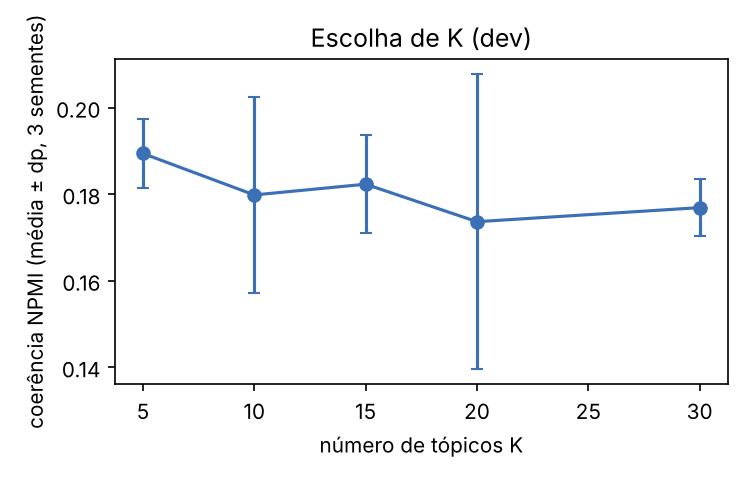
\includegraphics[width=0.42\linewidth]{figs/topicos_coerencia.png}\hfill
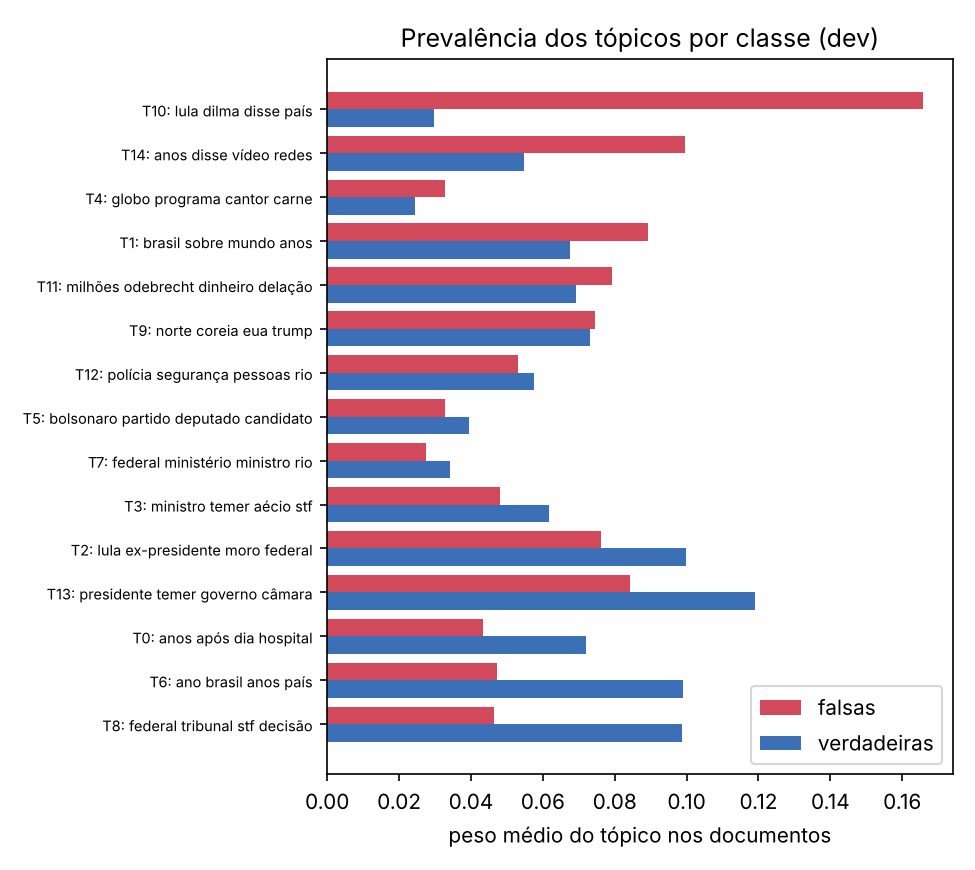
\includegraphics[width=0.55\linewidth]{figs/topicos_por_classe.png}
\caption{Esquerda: coerência NPMI por número de tópicos (média $\pm$ dp de 3 sementes). Direita:
peso médio de cada tópico nas falsas e nas verdadeiras.}\label{fig:topics}
\end{figure}

A coerência quase não varia entre $K=5$ e $K=30$ (Tabela~\ref{tab:k}); as diferenças são da ordem
da variação entre sementes. Escolhemos o maior $K$ cuja coerência fica a menos de um desvio-padrão
da melhor, por analogia com a regra de um erro-padrão~\cite{breiman1984}, o que dá $K=15$ e tópicos
mais finos e interpretáveis. Esta regra foi aplicada depois de observar a curva, o que declaramos
como limitação.

\begin{table}[t]\centering\small
\caption{Escolha do número de tópicos: coerência NPMI média (3 sementes) e perplexidade.}\label{tab:k}
\begin{tabular}{rccc}
\toprule
K & NPMI & dp & Perplexidade \\
\midrule
5 & 0,189 & 0,008 & 3202 \\
10 & 0,180 & 0,023 & 3102 \\
15 & 0,182 & 0,011 & 3133 \\
20 & 0,174 & 0,034 & 3190 \\
30 & 0,177 & 0,007 & 3298 \\
\bottomrule
\end{tabular}
\end{table}

\begin{table}[t]\centering\scriptsize
\caption{Os 15 tópicos LDA (dev), ordenados do mais típico das falsas ao mais típico das verdadeiras.}\label{tab:topics}
\begin{tabular}{lrrrp{4.6cm}}
\toprule
Tóp. & F/V & \%F & Docs & Termos mais prováveis \\
\midrule
T10 Críticas a Lula e ao PT & 5,60 & 93 & 606 & lula dilma disse país vai \\
T14 Histórias familiares e redes sociais & 1,82 & 69 & 454 & anos disse vídeo redes sobre \\
T4 TV Globo e celebridades & 1,35 & 60 & 103 & globo programa cantor carne apresentador \\
T1 Conspirações e temas gerais & 1,32 & 52 & 456 & brasil sobre mundo anos país \\
T11 Delações e corrupção (Odebrecht) & 1,14 & 60 & 443 & milhões odebrecht dinheiro delação empresa \\
T9 Coreia do Norte e EUA & 1,02 & 48 & 432 & norte coreia eua trump kim \\
T12 Polícia e incidentes & 0,92 & 47 & 294 & polícia segurança pessoas rio policiais \\
T5 Eleições de 2018 & 0,83 & 45 & 161 & bolsonaro partido deputado candidato psdb \\
T7 Segurança pública e governo & 0,80 & 42 & 113 & federal ministério ministro rio presos \\
T3 Temer, Aécio e tribunais & 0,78 & 43 & 312 & ministro temer aécio stf senador \\
T2 Lava Jato: Lula e Moro & 0,76 & 43 & 536 & lula ex-presidente moro federal jato \\
T13 Governo Temer e Congresso & 0,71 & 38 & 682 & presidente temer governo câmara michel \\
T0 Acidentes e quotidiano & 0,60 & 34 & 327 & anos após dia hospital ano \\
T6 Saúde e estatísticas & 0,48 & 29 & 419 & ano brasil anos país mil \\
T8 Decisões judiciais & 0,47 & 27 & 418 & federal tribunal stf decisão justiça \\
\bottomrule
\end{tabular}\par\smallskip{\footnotesize NMI(tópico dominante, classe) = 0,047; NMI(tópico dominante, tema) = 0,104. Razão F/V: peso médio do tópico nas falsas a dividir pelo peso nas verdadeiras.}
\end{table}


Dois tópicos concentram as falsas (Tabela~\ref{tab:topics}): \emph{Críticas a Lula e ao PT}
(T10), com peso 5,6 vezes maior nas falsas e 93\% de falsas entre os documentos onde domina, e
\emph{Histórias familiares e redes sociais} (T14). Os documentos mais representativos de T10 têm
marcas opinativas e sensacionalistas (``CRIME!'', ``roubalheira''). Do lado das verdadeiras estão as
\emph{Decisões judiciais} (T8), \emph{Saúde e estatísticas} (T6) e \emph{Acidentes e quotidiano}
(T0). Nem todos os tópicos têm um tema único: \emph{Conspirações e temas gerais} (T1) junta teorias da
conspiração a textos genéricos sobre o Brasil e o mundo. Ainda assim, o tópico dominante está mais
associado ao tema do corpus (NMI 0,104) do que à veracidade (0,047), e uma regressão logística sobre
as 15 proporções de tópicos obtém apenas 0,747 de F1-macro [0,736; 0,758].

\subsection{Extração de informação}

\begin{table}[t]\centering\scriptsize
\caption{Extração de informação: avaliação no ouro anotado manualmente.}\label{tab:ieeval}
\begin{tabular}{llccccr}
\toprule
Correspondência & Tipo & P & R & F1 & IC95\% & $n$ ouro \\
\midrule
estrita & PESSOA & 0,776 & 0,909 & 0,837 & [0,806; 0,865] & 396 \\
estrita & ORGANIZACAO & 0,681 & 0,409 & 0,511 & [0,457; 0,562] & 303 \\
estrita & LOCAL & 0,377 & 0,938 & 0,537 & [0,464; 0,603] & 130 \\
estrita & DATA & 0,716 & 0,765 & 0,739 & [0,650; 0,821] & 102 \\
estrita & TODOS (micro) & 0,634 & 0,735 & 0,681 & [0,653; 0,710] & 931 \\
relaxada & PESSOA & 0,841 & 0,965 & 0,898 & [0,874; 0,920] & 396 \\
relaxada & ORGANIZACAO & 0,725 & 0,429 & 0,539 & [0,485; 0,588] & 303 \\
relaxada & LOCAL & 0,410 & 0,954 & 0,574 & [0,498; 0,639] & 130 \\
relaxada & DATA & 0,881 & 0,922 & 0,901 & [0,852; 0,944] & 102 \\
relaxada & TODOS (micro) & 0,696 & 0,784 & 0,737 & [0,711; 0,762] & 931 \\
\bottomrule
\end{tabular}\par\smallskip{\footnotesize Concordância entre anotadores (F1, 20 docs): 0,875 estrita, 0,931 relaxada.}
\end{table}

\begin{table}[t]\centering\small
\caption{Densidade de entidades por 100 palavras (dev, texto normalizado, \texttt{pt\_core\_news\_md} + regras para datas). Teste de Wilcoxon emparelhado por par ($n=2\,878$).}\label{tab:iedens}
\begin{tabular}{lcccc}
\toprule
Medida & Falsas & Verdadeiras & Mediana F$-$V & $p$ \\
\midrule
Pessoas & 3,99 & 3,33 & 0,48 & $<10^{-4}$ \\
Organizações & 1,42 & 1,57 & 0,00 & 0,0001 \\
Locais & 2,43 & 3,28 & -0,72 & $<10^{-4}$ \\
Datas & 0,43 & 1,28 & -0,73 & $<10^{-4}$ \\
Expressões de atribuição & 0,75 & 0,50 & 0,00 & $<10^{-4}$ \\
\bottomrule
\end{tabular}
\end{table}


No ouro (Tabela~\ref{tab:ieeval}), o extrator tem F1 global de 0,681 (precisão 0,634, revocação
0,735), abaixo da concordância entre anotadores (0,875). As pessoas são o tipo mais fácil (0,837) e as
datas ficam em 0,739. Os locais têm revocação alta (0,938) mas precisão muito baixa (0,377), e as
organizações o inverso (revocação 0,409). A causa é a mesma: o modelo etiqueta instituições como
locais. Das previsões erradas de LOCAL, 103 são organizações no ouro, com destaque para ``STF''
(15 vezes), ``Supremo Tribunal Federal'', ``Congresso'', ``PF'' e ``Ministério Público Federal''.
Ignorando o tipo, o F1 sobe para 0,818: o extrator encontra as entidades, mas erra a sua classe.

Este erro tem consequências na análise. Aplicado a todo o dev (Tabela~\ref{tab:iedens}), o extrator
sugere que as verdadeiras têm mais datas (1,28 vs.\ 0,43 por cem palavras) e mais locais (3,28 vs.\
2,43), e as falsas mais pessoas e mais expressões de atribuição (0,75 vs.\ 0,50). Com a anotação
humana dos 50 pares (Tabela~\ref{tab:iegold}), só a diferença nas \textbf{datas} se confirma, e
até se acentua: 1,24 vs.\ 0,23, cerca de cinco vezes mais nas verdadeiras ($p<10^{-4}$). A
diferença nos locais (1,02 vs.\ 0,69) deixa de ser significativa ($p=0{,}067$): era em grande parte
o efeito de as verdadeiras citarem mais instituições, que o extrator tomava por locais.

\begin{table}[t]\centering\small
\caption{Entidades por 100 palavras segundo a anotação HUMANA (50 pares do dev). Wilcoxon emparelhado por par.}\label{tab:iegold}
\begin{tabular}{lcccc}
\toprule
Tipo & Falsas & Verdadeiras & V/F & $p$ \\
\midrule
Pessoas & 2,82 & 2,48 & 0,9 & 0,124 \\
Organizações & 1,84 & 2,31 & 1,3 & 0,415 \\
Locais & 0,69 & 1,02 & 1,5 & 0,067 \\
Datas & 0,23 & 1,24 & 5,4 & $<10^{-4}$ \\
\bottomrule
\end{tabular}
\end{table}


% Responsáveis: P4 (análise de falhas) + todos (conclusões acionáveis) + P2/P3 (custo)
\section{Discussão}\label{sec:discussao}

\subsection{Análise de falhas}
Como o BERTimbau afinado erra apenas 19 notícias do teste, analisámos todos esses erros e
completámos a amostra com 21 erros do melhor modelo clássico (caracteres com SVM afinado), num total
de 40 (20 de cada tipo). Nove notícias foram mal classificadas pelos dois modelos.
A Tabela~\ref{tab:errors} mostra as categorias. Os falsos negativos (12) são todos notícias
\emph{falsas com estilo jornalístico}: datas, cargos entre parênteses, instituições e fontes citadas,
como a notícia falsa sobre o depoimento de Lula à Polícia Federal (E10). Os falsos positivos
dividem-se entre notícias verdadeiras \emph{com tom de opinião ou citações} (8), como uma reportagem
sobre terraplanistas que começa só com as palavras deles (E02), e notícias verdadeiras sobre
\emph{temas típicos das falsas} (7), como polémicas de celebridades ou Lula e a Lava Jato (E03, E08).

Os dois modelos erram de forma diferente. O modelo clássico falha sobretudo por pistas
superficiais: o tema (6 de 21) e o estilo jornalístico imitado (8 de 21). O BERTimbau, que capta
melhor o tom, falha sobretudo em textos verdadeiros de opinião ou análise (5 dos 10 erros só
seus), que associa às notícias falsas. Entre os 9 erros comuns, 3 parecem \emph{erros de rótulo
no corpus}: notícias reais copiadas por sítios de desinformação, algumas ainda com a assinatura da
agência ou do jornal de origem (``agências/R7'', ``O Tempo''). No total, 5 dos 40 erros têm
rótulo duvidoso, o que sugere que parte do ``erro'' restante do BERTimbau é ruído do próprio corpus,
rotulado pelo sítio de origem e não pela veracidade de cada notícia. Por fim, 4 erros vêm de textos
quase vazios (9 a 20 palavras no corpus), sem informação suficiente para decidir.
\todo{P4: rever este comentário (categorias de E10--E40 sugeridas pelo assistente)}

\begin{table}[t]\centering\scriptsize
\caption{Categorias de erro do melhor modelo no teste (40 erros analisados). FP: verdadeira classificada como falsa; FN: falsa classificada como verdadeira.}\label{tab:errors}
\begin{tabular}{lrrrl}
\toprule
Categoria & FP & FN & Total & Exemplos \\
\midrule
Falsa com estilo jornalístico & 0 & 12 & 12 & E09, E10, E15 \\
Verdadeira com tom de opinião ou citações & 8 & 0 & 8 & E02, E06, E13 \\
Tema típico da outra classe & 7 & 0 & 7 & E03, E04, E08 \\
Possível erro de rótulo no corpus & 0 & 5 & 5 & E07, E12, E14 \\
Pouco texto informativo no corte & 1 & 3 & 4 & E01, E05, E26 \\
Outro & 3 & 0 & 3 & E17, E25, E33 \\
Marcas da fonte & 1 & 0 & 1 & E18 \\
\bottomrule
\end{tabular}
\end{table}


\subsection{Resposta à pergunta da organização}
Os três tipos de análise apontam na mesma direção: no Fake.Br, o que distingue as notícias falsas
é \emph{como} são escritas (frases curtas, registo informal, erros, ausência de datas
concretos), e não \emph{de que} falam. Daqui retiramos três conclusões acionáveis:
\begin{enumerate}
\item \textbf{Não confiar em métricas que o comprimento explica.} Qualquer avaliação de um detetor
deve incluir a \emph{baseline} de comprimento; no Fake.Br ela atinge 0,944.
\item \textbf{Usar a ausência de datas como sinal de triagem.} As verdadeiras têm cerca de cinco
vezes mais datas concretas, confirmado com anotação humana. Notícias sem nenhuma data devem subir na
fila de verificação. É um sinal simples, explicável ao verificador e menos dependente do tema; um
extrator de entidades genérico não basta para os outros tipos, porque confunde instituições com locais.
\item \textbf{Usar o BERTimbau afinado como detetor principal e os n-gramas de caracteres como
alternativa barata.} O primeiro é o mais exato mesmo sem atalhos (0,987); o segundo corre em CPU,
generaliza melhor do que as palavras para temas novos e explica-se com os atributos mais pesados.
Em ambos os casos, reavaliar periodicamente, porque o desempenho em temas não vistos cai até 5,5 pontos.
\end{enumerate}
As três conclusões mantêm-se no teste (Tabela~\ref{tab:test}).

\subsection{Custo computacional}
A Tabela~\ref{tab:cost} resume o custo dos modelos finais, medido com o mesmo protocolo
(\texttt{src/cost.py}) num computador com Windows~11, processador AMD de 16 núcleos lógicos e 15\,GB de
RAM. Os modelos clássicos treinam em 10 a 43\,s, ocupam no máximo 3,5\,MB e classificam uma notícia
em 1 a 11\,ms, com menos de 200\,MB de memória. O extrator de entidades (\texttt{md}) processa cada
notícia em cerca de 36\,ms; o modelo \texttt{lg} tem mais 577\,MB do que o \texttt{md} para um
ganho de 1,6 pontos de F1 (Secção~\ref{sec:metodo}). O BERTimbau precisa de GPU: no Colab gratuito
(T4), o \emph{fine-tuning} com 5 folds demorou 12 minutos com 3,6\,GB de memória, e o treino final
mais a previsão das 1\,444 notícias de teste 167\,s; o modelo ocupa cerca de 436\,MB. Os cinco
pontos de F1 que o BERTimbau ganha aos modelos clássicos custam, portanto, uma GPU e um modelo cerca
de cem vezes maior. O pipeline não usa modelos de linguagem nem serviços externos pagos (0 tokens,
0 euros); o único recurso externo foi a GPU gratuita do Colab.

\begin{table}[t]\centering\scriptsize
\caption{Custo computacional. Treino no dev completo (5\,756 notícias); inferência medida em 1\,000 notícias. Memória: pico de RAM do processo (GPU no caso do BERTimbau). CPU: Windows 11, 16 núcleos lógicos, 14,9 GB de RAM; GPU: Google Colab gratuito. Nenhum serviço externo pago nem modelo de linguagem foi usado no pipeline (0 tokens).}\label{tab:cost}
\begin{tabular}{llrrrr}
\toprule
Modelo & Hardware & Treino (s) & ms/notícia & Memória (MB) & Tam. (MB) \\
\midrule
Só comprimento & CPU & 0,0 & 0,00 & 0 & 0,0 \\
palavras + SVM & CPU & 10,1 & 1,45 & 110 & 3,5 \\
caracteres + SVM & CPU & 39,5 & 10,83 & 129 & 1,5 \\
caracteres + LogReg & CPU & 42,7 & 10,86 & 175 & 3,0 \\
spaCy (md) & CPU & -- & 36,44 & 284 & 54,1 \\
BERTimbau afinado: CV 5 folds & GPU T4 & 713,2 & -- & 3587 & 436,0 \\
BERTimbau afinado: final + teste & GPU T4 & 167,4 & -- & 3580 & 436,0 \\
\bottomrule
\end{tabular}
\end{table}


% Responsável: P1 (base legal verificada em 17/11/2026; rever a redação)
\section{Considerações éticas e limitações}\label{sec:etica}

\paragraph{Dados pessoais (RGPD).}
As notícias identificam pessoas reais, sobretudo figuras públicas, e associam-nas a partidos e
posições políticas. Dados que revelem opiniões políticas são uma categoria especial cujo tratamento
o RGPD proíbe em regra (art.~9.º, n.º~1)~\cite{rgpd2016}. Duas exceções do n.º~2 cobrem o nosso uso:
a alínea~e), para dados manifestamente tornados públicos pelo titular, como as declarações públicas
de políticos, e a alínea~j), para fins de investigação científica, com as garantias do art.~89.º.
Algumas notícias mencionam também pessoas privadas (vítimas, familiares, uma criança), e várias
notícias falsas fazem acusações difamatórias. Medidas adotadas: não redistribuímos os textos (o
código descarrega-os da fonte); não construímos perfis de pessoas; no artigo citamos apenas excertos
curtos e, quando possível, descrevemos os casos sem nomes. Os modelos guardam vocabulário, incluindo
nomes próprios, pelo que um sistema em produção deveria minimizar esses atributos e fazer uma
avaliação de impacto sobre a proteção de dados antes de ser usado.

\paragraph{Licença.}
O repositório do corpus não tem ficheiro de licença; os autores pedem apenas a citação dos artigos
de origem. Usamo-lo para investigação académica, sem redistribuir os dados.

\paragraph{Enviesamentos.}
(1)~\emph{Político}: 58\% do corpus é política, e o tópico mais associado às notícias falsas é dominado
por ataques a figuras de um só partido (\emph{Críticas a Lula e ao PT}, T10). Um modelo pode aprender
a associar o vocabulário de um quadrante político à falsidade e penalizar notícias verdadeiras sobre
esses temas, como sugerem os falsos positivos da categoria \emph{Tema típico da outra classe}.
(2)~\emph{De fonte}: 93\% das falsas vêm de um único sítio e quase todas as verdadeiras de três grupos
de comunicação; parte do ``estilo'' aprendido pode ser o estilo editorial desses sítios, como
Potthast et~al.~\cite{potthast2018} alertam. A análise de erros mostra o reverso: notícias reais
copiadas por sítios de desinformação ficam rotuladas como falsas. (3)~\emph{Temporal e linguístico}:
as notícias são de 2016--2018 e em português do Brasil; o vocabulário político muda, e o desempenho
em notícias portuguesas não foi avaliado.

\paragraph{Riscos de utilização indevida.}
Usado como juiz automático, e não como apoio à triagem, o sistema poderia levar à remoção de conteúdo
legítimo (falsos positivos), por exemplo artigos de opinião verdadeiros, que são o erro mais comum do
BERTimbau, ou dar uma falsa sensação de segurança (falsos negativos). Quem produz desinformação pode
imitar o estilo jornalístico, incluindo datas e fontes, para escapar à deteção: é exatamente o que
acontece nos 12 falsos negativos analisados. Por isso, a decisão final deve caber sempre a um
verificador humano.

\paragraph{Nível de risco no Regulamento da IA.}
O Regulamento (UE) 2024/1689~\cite{aiact2024}, alterado pelo Regulamento (UE)
2026/1744~\cite{omnibus2026}, classifica como sistemas de risco elevado os usos do Anexo~III:
biometria, infraestruturas críticas, educação, emprego, serviços essenciais, aplicação da lei,
migração, justiça e processos democráticos. O Anexo~III não inclui a verificação de factos, a
moderação de conteúdos nem a deteção de desinformação; o ponto mais próximo, 8.b), refere sistemas
destinados a influenciar o resultado de eleições ou o comportamento dos eleitores, o que não é o caso
de uma ferramenta interna que ordena notícias para verificação humana. O sistema também não gera
conteúdos, pelo que as obrigações de transparência do art.~50.º não se aplicam. Segundo a nossa
leitura, trata-se portanto de um sistema de risco mínimo. A classificação deveria ser revista se o
sistema passasse a decidir sozinho a remoção de conteúdos ou fosse usado em contexto eleitoral; nesse
caso, a remoção por plataformas em linha está também sujeita ao Regulamento dos Serviços
Digitais~\cite{dsa2022}. Esta análise não substitui um parecer jurídico.

\paragraph{Limitações.}
O corpus é de um só país, período e conjunto de fontes; tem textos quase vazios e alguns rótulos
duvidosos; a regra de escolha de $K$ foi decidida após ver a curva de coerência; os atributos de
estilo do corpus foram calculados sobre o texto completo; a versão cortada reduz algumas notícias a
um título; e a avaliação da extração de informação assenta em 100 documentos sem adjudicação entre
anotadores.

% Responsável: todos
\section{Conclusões e trabalho futuro}\label{sec:conclusao}

Mostrámos que, no Fake.Br, o desempenho elevado dos detetores de notícias falsas se deve em grande
parte a um atalho, o comprimento, e que, removido esse atalho, os sinais que resistem são de estilo
e de ancoragem factual, não de tema. As três tarefas (classificação, tópicos e extração de
entidades) convergem nesta conclusão. No conjunto de teste, usado uma única vez, o BERTimbau afinado
na versão sem atalhos obtém F1-macro de 0,987 [0,980; 0,992], contra 0,939 do melhor modelo
clássico e 0,938 do comprimento, e as datas concretas, confirmadas por anotação manual, são o sinal
mais simples e explicável para a triagem.

Como trabalho futuro propomos: avaliar noutro corpus e período, sem o viés de fonte; comparar com
um modelo de linguagem em modo \emph{zero-shot}, controlando a possível contaminação dos dados de
treino com notícias de 2016--2018; e testar a robustez a falsas que imitem o estilo jornalístico.


\bibliographystyle{splncs04}
\bibliography{references}

% ---------------- Anexos: depois das referências, fora do limite de páginas ----------------
\appendix
% Anexo obrigatório (fora do limite de páginas). Os deltas têm de SOMAR 0,00.
\section{Avaliação pelos pares}\label{app:pares}

O grupo tem cinco elementos, composição autorizada pela docente.
A avaliação foi decidida em conjunto por todos os elementos.

\begin{center}
\begin{tabular}{llr}
\toprule
Número & Nome & Delta \\
\midrule
PG63946 & Diogo Filipe Oliveira Gomes & 0,00 \\
PG63711 & Sérgio Paulo Vieira Carvalho & 0,00 \\
PG64175 & Hugo Novais Martins & 0,00 \\
PG64174 & Diogo Valério Borges & 0,00 \\
PG64031 & Tiago Alexandre Lopes Mendes & 0,00 \\
\midrule
 & \textbf{Soma} & \textbf{0,00} \\
\bottomrule
\end{tabular}
\end{center}
Todos os elementos contribuíram de forma equivalente para o trabalho, pelo que o grupo atribuiu
um delta nulo a cada um.

% Anexo obrigatório (fora do limite de páginas): ferramentas, para quê, e um caso em que errou.
\section{Declaração de utilização de assistentes de IA}\label{app:ia}

\paragraph{Ferramentas e finalidade.}
Usámos o assistente Claude para: gerar a primeira versão do código do repositório (carregamento,
divisão, pré-processamento, classificação, tópicos, extração de informação e \emph{notebook} do
BERTimbau); explicar alguns conceitos; redigir um esqueleto deste
artigo; e apoiar a interpretação de alguns resultados, que o grupo reviu e validou. A anotação manual dos 100
documentos para a extração de informação foi feita exclusivamente pelos cinco elementos do grupo. O
assistente esclareceu dúvidas sobre as regras do guia. Todas as decisões foram discutidas pelo
grupo, o código foi executado e verificado nos nossos computadores e o texto foi revisto e reescrito
por nós. Não foram usadas outras ferramentas de inteligência artificial.

\paragraph{Casos em que o assistente errou e como demos por isso.}
\begin{enumerate}
\item \textbf{Versão incompatível de uma biblioteca.} O \texttt{requirements.txt} inicial fixava o
\texttt{scikit-learn} 1.5.2, que não tem pacote pré-compilado para Python 3.14 no Windows. Demos
por isso quando um elemento do grupo tentou instalar o ambiente e a compilação falhou. A correção
(versão 1.7.2) foi validada a confirmar que todas as tabelas davam exatamente os mesmos números.
\item \textbf{Pressuposto errado sobre os dados.} A primeira versão do carregador assumia que a
versão normalizada do corpus tinha exatamente os mesmos ficheiros que a versão completa; o código
falhou em quatro ficheiros com numeração diferente.
\item \textbf{Erros de programação apanhados por testes.} O \emph{notebook} do BERTimbau gravava os
identificadores num formato que o \texttt{numpy} recusa ler, e o gerador de tabelas usava um nome
de coluna (\texttt{pipe}) que coincide com um método do \texttt{pandas}. Ambos foram detetados ao
correr o código (o \emph{notebook} foi testado de ponta a ponta com um modelo minúsculo antes de
gastar GPU). Também um comentário acrescentado pelo assistente ao script do custo computacional
partiu uma linha de código (\texttt{SyntaxError}), o que só detetámos ao correr o script no Windows.
\end{enumerate}


\end{document}
